\section{Grafica pentru Miss Pacman}
% enuntul intrebarii
În această secțiune vom prezenta implementarea grafică a Miss Pacman.
\newline

\subsection{Draw Miss Pacman}
Pentru a o desena pe Miss Pacman am folosit modelul de grafică pentru fantome, dar în loc de două cercuri pentru doi ochi, va avea 2 cercuri pentru unul, si vor fi unul peste altul, de dimensiuni diferite. De asemenea Miss Pacman are o fundă mov care nu putea lipsi din designul nostru. \newline

\textbf{Cod din GraphicDesign:}
% a se completa fisierul code/mspacman.py
\inputminted[linenos]{python}{code/mspacman.py}

\begin{figure}[h]
    \centering
    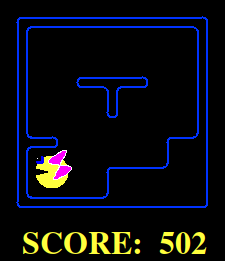
\includegraphics[width=6cm]{text/images/miss pacman.png}\\
    \caption{Miss Pacman}
\end{figure}


\vspace{0.75cm}
\pagebreak
